\documentclass[11pt]{article}
%بسم الله الرحمن الرحیم

%You should edit DSLecture.tex, not this file!

\usepackage{graphicx}
\usepackage{amsthm}
\usepackage{latexsym}
\usepackage{amssymb}
\usepackage{verbatim}
\usepackage{enumitem,array}
\usepackage{multirow}
\usepackage{blindtext}
\usepackage{tikz}
\usepackage{tkz-graph}
\usepackage{bookmark}
\usetikzlibrary{automata,positioning,arrows, positioning,chains,fit,shapes,calc}
\usepackage[a4paper, margin=0.7in]{geometry}
\usepackage{listings}
\usepackage{clrscode3e}
\usepackage{etex}
\usepackage{hyperref}
\usepackage{etex}
\reserveinserts{28}
\hypersetup{
	colorlinks=true,
	linkcolor=blue,
	filecolor=magenta,      
	urlcolor=cyan,
}
\usepackage{xepersian}


\settextfont{HM XNiloofar}
\setlatintextfont{Lucida Sans}
%\setdigitfont{HM XNiloofar}
%\setdigitfont{ParsiDigits}
\defpersianfont\outline[Scale=1]{HM XNiloofar Outline}

\setlength{\parindent}{1.5em}
\setlength{\parskip}{0.9em}
\renewcommand{\baselinestretch}{1.4}


\newcommand{\lecture}[3]{
	%\pagestyle{empty}
	{
		\begin{center}
			\vspace{-1cm}
			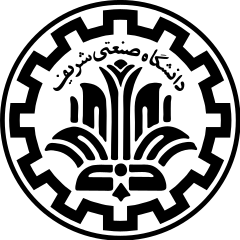
\includegraphics[scale=0.15]{Sharif}%\hfill \\[1em]  
		\end{center}
		\vspace{-8mm}
		\begin{center}
			
			\bf
			%\begin{outline} 
			{
				\Large
سمینار آنالیز عددی 
			}
			%\end{outline} 
			\\
مدرس: قهرمان طاهریان
			\\~
		\date{\today}
		\end{center}
	}\vspace*{-1em}
	\noindent
 #1: #2 \hfill نگارنده: #3
	\vspace{-4mm}
	\rule{\textwidth}{1pt}
	\ \\
}

% example environment
\newenvironment{example}
{\smallskip \noindent \emph{مثال:}}
{\hfill $\boxtimes$ \smallskip}


\newtheorem{theorem}{قضیه}
\newtheorem{proposition}{گزاره}
\newtheorem{claim}{ادعا}
\newtheorem{lemma}{لم}
\newtheorem{corollary}{نتیجه}
\newtheorem{definition}{تعریف} % Use this for non-trivial definitions.


	
\begin{document}
	\lecture{عنوان}{QUASI-NEWTON}{صالح مومنی و نیما بهرنگ}
	مروری کوتاه بر آن‌چه گذشت و مقدمه‌ای کوتاه بر مطالب این جلسه. 
	
	\section{عنوان بخش}
	شروع بحث جلسه فعلی. 
	
	پاراگراف‌ها با یک خط خالی از هم جدا می‌شوند. 
	
	سعی کنید قواعد نگارش فارسی را رعایت کنید. از نیم‌فاصله
	به درستی استفاده کنید. علامت نقل قول در فارسی بدین صورت است «». پس از نقطه و ویرگول و دونقطه و پرانتزبسته‌ای که قبل از نقطه نیست و این‌گونه علامت‌ها، یک فاصله بگذارید.
	
	خوب است معادل انگلیسی اصطلاحات را در پاورقی%
	\LTRfootnote{footnote}
	بیاورید.
	
	برای نوشتن انگلیسی در میان متن فارسی، از دستور \verb+\lr{}+ استفاده کنید. 
	مثلا:
	\lr{Some English text here} 
	در میان متن درست می‌آید.
	
	استفاده از تاکید به صورت 
	\textbf{پررنگ}
	کردن یا 
	\textit{ایتالیک}
	کردن مفید است. 
	
	برای استفاده از یک کلمه (انگلیسی) در محیط ریاضی، حتما از دستور
	\lr{\textbackslash text}
	استفاده کنید (مثال شبه‌کد را ببینید). 
	
	یک سایت خوب راهنمای لاتک سایت 
	\url{https://www.overleaf.com/}
	است. 
	راهنمای مقدماتی لاتک این سایت را می‌توانید در 
	\href{https://www.overleaf.com/learn/latex/Learn_LaTeX_in_30_minutes}{اینجا}
	مشاهده کنید. 
	همچنین برای نوشتن فرمول‌های چندخطی  
	\href{https://www.overleaf.com/learn/latex/Aligning_equations_with_amsmath}{اینجا}
	را ببینید. 
	
	برای شبه کدها از پکیج
	\lr{clrscode3e}
	استفاده کنید. برای آشنایی با این پکیج
	\lr{clrscode.pdf}
	را مطالعه کنید.
		\begin{latin}
		\begin{codebox}
		\Procname{$\proc{DVDSelect}(A,n)$}

		\end{codebox}
	\end{latin}
	
	
	
	\section{محیط‌های مختلف}
	\begin{lemma}
		یک لم.
	\end{lemma}
	\begin{theorem}
		\label{thm:sample}
		یک قضیه. 
	\end{theorem}
	\begin{proof}
		بدیهی.
	\end{proof}
	
	\begin{example}
		یک مثال. 
	\end{example}
	
	ارجاع به قضیه 
	\ref{thm:sample}.
	
	ارجاع به مراجع
	\cite{persianreference}
	و
	\cite{CLRS}.
	
	%برای قاطی نشدن متن فارسی و انگلیسی از
	% Enter
	%  زیاد استفاده کنید!
	
	\bibliographystyle{alpha}
	
	\begin{thebibliography}{99}
		\bibitem{persianreference}
		مرجع فارسی. 
		
		\begin{latin}	%english references
			
			%book in MLA style: https://owl.purdue.edu/owl/research_and_citation/mla_style/mla_formatting_and_style_guide/mla_works_cited_page_books.html
			\bibitem{CLRS} %english reference example. 
			Cormen, Thomas H., et al.
			\textit{Introduction to Algorithms}. 
			3rd ed., MIT Press, 2009, pp. 18-22. %page numbers
		\end{latin}	
	\end{thebibliography}
	\pagebreak
\end{document}


